%
% Einfache LaTeX-Vorlage für Arbeiten am Lehrstuhl Kranzlmüller / MNM-Team
% - optimiert für die Arbeit mit gängigen LaTeX-Editoren
% - funktioniert ohne Makefile und Anpassungen der LaTeX-Verzeichnisstruktur
% - verwendet Komaskript für ein (nach europäischen Gepflogenheiten) schöneres Layout
% 
% v1, 2007 (Michael Brenner)
% v1.1, 2012 (Michael Brenner)
% v1.2, 2017 (Michael Brenner)
% v1.2.1, 2017 (Benjamin Schnoy)
% Diese Version: v1.2.2, 2019 "Robin Lösch <robin@chilio.net>"
% Entfernen von OSX spezifischen Files
% Konvertierung auf UTF8
% Entfernen von executable bits auf text Files

\documentclass[bibliography=totoc,listof=totoc,BCOR=5mm,DIV=12]{scrbook} % Rand für Bindung: 5mm / falls Index verwendet, ergänze "index=totoc" zu den Optionen 
%\usepackage{ngerman} % Trennung nach neuer deutscher Rechtschreibung, deutsche Sonderzeichen, z.B. \glqq und \grqq für deutsche Anführungszeichen 
\usepackage[utf8]{inputenc} % Umlaute im Text
\usepackage{graphicx} % Einfügen von Grafiken  - für PDF-Latex: .pdf und .png (.jpg möglich, sollte aber vermieden werden)
\usepackage{url}           % URL's (z.B. in Literatur) schöner formatieren
\usepackage{hyperref} % sorgt für für Hyperlinks in PDF-Dokumenten

\graphicspath{{./images/}}

%custom symbols
\usepackage{xcolor}
\usepackage{pifont}
\newcommand{\degree}{$^{\circ}$ }
\newcommand{\ar}{$\rightarrow$ }
\definecolor{forestgreen}{rgb}{0.13, 0.55, 0.13}
\definecolor{cadmiumred}{rgb}{0.89, 0.0, 0.13}
\newcommand{\checkm}{\textcolor{forestgreen}{\ding{51}}}
\newcommand{\cross}{\textcolor{cadmiumred}{\ding{55}}}


\usepackage{amsmath}
\usepackage[prependcaption,textsize=tiny]{todonotes} %TODO remove before end
\usepackage{hyperref}
\usepackage{subcaption}
%\usepackage{lstlisting}
\usepackage{verbatim} %TODO remove before end
\usepackage{multirow}

\setcounter{secnumdepth}{2} %counter depth for subsubsections
\setcounter{tocdepth}{1} %list of contents depth 

\input{hyphenation} % in dieses File kommen Wörter die Latex nicht richtig trennt

\begin{document}

% ---------------------------------------------------------------
\frontmatter % Titelblätter und Erklärung
    %%%%%%%%%%%%%%%%%%%%%%%%%%%%%%%
% erste Seite
\let\textacute\'

\thispagestyle{empty}

\begin{center}

\vspace*{-2cm}

{\Huge INSTITUT FÜR INFORMATIK\\[1mm]}
DER LUDWIG--MAXIMILIANS--UNIVERSITÄT MÜNCHEN\\

\vspace*{1cm}

\includegraphics[width=0.3\textwidth]{lmu_siegel}

\vspace*{2cm}

{\Large \textbf{Master's Thesis}}\\ % oder Fortgeschrittenenpraktikum, Master's Thesis, Bachelorarbeit etc.

\vspace{2.0cm}
{\Huge \textbf{Pixel-based image synthesis}}\\
\vspace*{3mm}
{\Huge \textbf{of 360\degree viewpoints}}\\
%\vspace*{3mm}
%{\Huge \textbf{-- Adipiscing Elit}}\\
\vspace{1.5cm}

{\LARGE Rosalie Kletzander} % Name des Autors

\vspace{3cm}
Draft vom \today % erleichtert den Betreuern die Zuordnung - für finale Version entfernen

\end{center}

\newpage

%%%%%%%%%%%%%%%%%%%%%%%%%%%%%%%
% zweite Seite

\thispagestyle{empty}
\cleardoublepage

%%%%%%%%%%%%%%%%%%%%%%%%%%%%%%%
% dritte Seite (Kopie der ersten)

\thispagestyle{empty}

\begin{center}

\vspace*{-2cm}

{\Huge INSTITUT FÜR INFORMATIK\\[1mm]}
DER LUDWIG--MAXIMILIANS--UNIVERSITÄT MÜNCHEN\\

\vspace*{1cm}

\includegraphics[width=0.3\textwidth]{lmu_siegel}

\vspace*{2cm}

{\Large \textbf{Master's Thesis}}\\ % oder Fortgeschrittenenpraktikum, SEP etc.

\vspace{2.0cm}
{\Huge \textbf{Pixel-based image synthesis}}\\
\vspace*{3mm}
{\Huge \textbf{of 360\degree viewpoints}}\\
%\vspace*{3mm}
%{\Huge \textbf{-- Adipiscing Elit}}\\
\vspace{1.5cm}

{\LARGE Rosalie Kletzander} % Name des Autors
\vspace{2cm}

\parbox{1cm}{
\begin{large}
\begin{tabbing}
Aufgabensteller: \hspace{.5cm} \=Prof. Dr. Dieter Kranzlmüller\\[2mm]
Betreuer:
\>Markus Wiedemann\\ % alphabetische Reihenfolge (Nachname)
\>Jean-Fran\c{c}ois Lalonde (Universit\textacute{e} Laval, Kanada)\\[5mm]%
Abgabetermin: \> 28. Januar 2021\\
\end{tabbing}
\end{large}}\\
\vspace{5mm}

\end{center}
 % Titelblätter LMU
    \thispagestyle{empty}
    \cleardoublepage
    \include{./cover/erklaerung-lmu} % Erklärung (Arbeit selbstständig verfasst)
    \thispagestyle{empty}
    \cleardoublepage
    \vspace*{2cm}

\begin{center}
    \textbf{Abstract}
\end{center}

\vspace*{1cm}

\noindent 
Virtual Reality technology allows users to experience virtual environments by interacting with them, and navigating within them. These environments tend to be either meticulously modeled in 3D by hand, or recorded using 360\degree cameras. The advantage of using 360\degree images is that a high level of realism is achievable with relatively little effort. However, the use of 360\degree images generally limits users to a single viewpoint or forces them to ``jump'' between different viewpoints.
In order to improve the viewing experience,
image-based rendering, or image-based synthesis, aims to create novel viewpoints based on captured viewpoints, in the best case enabling a user to navigate freely and naturally within a scene.
There are a number of different approaches to image-based synthesis, many of which use some form of feature correspondence to extract
%information from the captured images.
 the scene geometry from the captured images.
While using the scene geometry makes it possible to synthesize novel views, it can also be problematic, since accurate scene geometry is very difficult to obtain unless dedicated depth sensors are used, and inaccurate scene geometry can lead to severe artefacts.

In order to reduce the number and severity of these artefacts,
this thesis proposes a pixel-based 2-DoF synthesis algorithm that combines basic reprojection with flow-based interpolation.
Instead of estimating scene geometry, a sphere is used as a proxy for inaccurately estimated scene geometry.
%which is similar to using incorrectly estimated geometry, in that it can lead to severe artefacts. 
%in place of estimated scene geometry makes it possible to synthesize novel views within a scene without knowledge about the geometry.
%However, the difference of the proxy geometry from the scene geometry can lead to severe artefacts.
To mitigate the artefacts caused by the inaccurate geometry, flow-based interpolation is used to generate viewpoints with more accurate perspectives in a method called ``flow-based blending''.
%The introduction of flow-based interpolation, which is generally leveraged for 1-DoF interpolation between pairs of images, aims to alleviate some of the artefacts by generating viewpoints with more accurate perspectives.
A proof-of-concept implementation of the approach is presented and tested with a select set of parameters, using different virtual and real scenes.
The synthesized images are then evaluated based on mathematical error metrics, as well as on visible artefacts. The results of the evaluation show that in the majority of cases where the basic method produces significant artefacts, the synthesis using flow-based blending improves the accuracy of the results.


 % Abstract
    \thispagestyle{empty}
    \tableofcontents % Inhaltsverzeichnis

% ---------------------------------------------------------------
\mainmatter % die eigentliche Arbeit

    \chapter{Introduction}

Virtual Reality, Augmented Reality and Computer Generated Imagery are ubiquitous in our increasingly digitalized world. Whether for immersive games played on head-mounted displays, image filters on social media, or movie productions involving special effects (which includes most), mixing virtual and real objects and worlds is not only accepted, it is often even expected.

A key factor to making the combination of the real and the virtual believable to human perception is correct lighting. If a virtual object in a real scene is not lit correctly, this is immediately recognizable by a human viewer, and breaks immersion. In order to ensure sufficient visual quality, lighting has to be meticulously captured in scenes that will contain clearly visible virtual objects. This tends to be done by substituting the virtual object by one or several spheres with different reflective characteristics (e.g. mirrored surface). Since this capture needs to be done manually at every desired point, capturing the lighting conditions at different points of a scene is very time-consuming.

In order to research how this process of capturing illumination can be improved, a project started in 2019 at the Laboratoire de Vision et Syst\` emes Num\' eriques (Laboratory for Computer Vision and Computer Systems, LVSN) at the Universit\'e Laval in Qu\'ebec, Canada aims to make illumination capture faster and more intuitive. 
%The goal of this project is to make the process of capturing illumination faster and more intuitive.
As a result, instead of having to place a reflective sphere at every location where illumination data is required, the capturer is able to walk around in the scene, carrying a 360$^{\circ}$ camera that is recording images of the surroundings. From this captured data, the lighting at each point in the room is extrapolated.

This process can be broken down to three distinct steps:
\begin{enumerate}
\item Capture of data with a 360$^{\circ}$ camera
\item Synthesis of non-captured viewpoints so that illumination can be estimated at \emph{every} point of the scene
\item Generation of high-dynamic range (HDR) data from low-dynamic range image data which can be directly used as illumination input to light virtual objects
\end{enumerate}

The synthesis of non-captured 360$^{\circ}$ viewpoints in step 2 is the focus of this thesis. This step is necessary so that the capturer is not required to record the scene from each possible point but can just record parts of the scene. The missing points can then be synthesized later, which saves capture time and memory space.

In general, there are several different approaches to view synthesis, which take into account different amounts of information on the 3D geometry of the scene. On one end of the scale, as much geometry information as possible is extracted from the image. However, using 3D geometric information requires very high-quality 3D data, which is difficult to recover from images. Lower-quality data tends to lead to visually unappealing results. \todo{citation?} Newer 3D geometry approaches use neural rendering, including Karimi et al.'s *name of paper/thesis*, which is also a part of the project at the LVSN.

Next come approaches that use only some 3D geometry information, such as depth layers, usually known as 2.5D. Here, the image is split into x different layers, each with a distinct depth. The objects in the scene are then each associated with one of the layers.

Approaches at the other end of the scale use no geometry whatsoever. Since there is no distinct name for this, the term used in this thesis is \emph{pixel-based rendering}, since the synthesis is based solely on pixels, disregaring any semantic information. \todo{taxonomy graphic}
Pixel-based rendering works fairly well for regular, planar images but has seen little or no research as of yet for 360$^{\circ}$ images. To start filling this research gap, this thesis explores the possibilities of adapting pixel-based rendering for panoramic image data. \todo{ok, now it's really important to make a clean gap analysis}

%In general, there are two fundamentally different approaches to view synthesis: using 3D geometric information of the scene, or using only the captured image data without any geometry. Using 3D geometric information requires very high-quality 3D data, which is difficult to recover from images. Lower-quality data tends to lead to visually unappealing results \todo{citation?}. Newer 3D geometry approaches use neural rendering, including Karimi et al.'s *name of paper/thesis*, which is also a part of the project at the LVSN. Synthesizing viewpoints \emph{without} using geometry, which is known as image-based rendering, works fairly well for regular, planar images but has seen little or no research as of yet for 360$^{\circ}$ images. To start filling this research gap, this thesis explores the possibilities of adapting image-based rendering for panoramic image data. \todo{ok, now it's really important to make a clean gap analysis}

\todo{logically from the text flow, this should go after the problem statement, even though it is part of the motivation.} In addition to its applicability for the lighting estimation project at the LVSN, the synthesis of non-captured 360$^{\circ}$ viewpoints has relevance on its own: Panoramic imagery is often used in Virtual Reality, for example for viewing historic locations and building interiors, or as a backdrop for VR games. The ability to accurately synthesize uncaptured viewpoints could greatly improve these viewing experiences, for example by creating stereo images or improving sample density for smoother navigation.

Furthermore, the results of this thesis can be combined with approaches using 3D geometry in order to leverage the advantages of both.

%
%- in addition to its necessity to the lighting estimation project, synthesizing non-captured viewpoints has relevance on its own
%--> there is a lot of research into improving VR viewing experiences
%--> most of it is based on using 3D geometry of the scene

\section*{Problem Statement}


The two distinct approaches in view synthesis (i.e. using no 3D geometry at all versus using as much 3D geometry as possible) have previously been researched for different applications:
Pixel-based rendering has been explored for planar (regular) images, for example to create smoothly viewable stereo panoramas from casually captured video input by Richardt et al. \cite{megastereo}, and there have been approaches to synthesising panoramic viewpoints from 360$^{\circ}$ video input by estimating 3D geometry, for example from Huang et a. \cite{6dof}. However, there is little to no research on using pixel-based rendering for synthesizing views from 360$^{\circ}$ image input. \todo{maybe include a collection of papers grouped into 4 areas: panoramic input, planar input, 3d geometry, pixel-based rendering. Definitely put this in, but not here}

%As mentioned above, there are two different approaches to view interpolation: Image-based rendering, and approaches using 3D geometry. Image-based rendering has been explored for planar (regular) images, for example to create smoothly viewable stereo panoramas from casually captured video input by Richardt et al. \cite{megastereo}, and there have been approaches to synthesising panoramic viewpoints from 360$^{\circ}$ video input by estimating 3D geometry, for example from Huang et a. \cite{6dof}. However, there is little to no research on using image-based rendering for synthesizing views from 360$^{\circ}$ image input. \todo{maybe include a collection of papers grouped into 4 areas: panoramic input, planar input, 3d geometry, image-based rendering. Definitely put this in, but not here}

In order to examine the potential of this approach, this thesis evaluates how well 360$^{\circ}$ panoramic view interpolation works when using image-based rendering without any supplemental geometric information i.e. pixel-based rendering.

Quality is difficult to quantify in the context of human perception, so the evaluation is based on different factors: euclidean distance to the ground truth, and visual believability. In this case, visual believability is measured by way of a minimal user study. In order to be able to compare the quality difference of the extension from planar to panoramic images, planar image results are also subjected to the same evaluation.

\section*{Scope}
%
%The development of your systematic took work. Now, leverage it!
%- in the methodology: do you vary parameters over some of them? in which steps?
%--> refer to here
%- in the definition of scope: how does the other work (other student,
%  literature, products) fit into this space? Where does yours?


Many different variables come into play when capturing image data, such as the metadata stored by the camera, the type of scene, the physical distance between captures, and much more. For the LVSN project, these variables do not need to be examined exhaustively, so the scope of this thesis is limited accordingly:

\paragraph{Location and rotation information}
Casually captured input data can be very unpredictable, as the capturer may move and rotate the camera freely. The captures used in this evaluation contain locational and rotational information in order to eliminate preprocessing steps such as simultaneous localization and mapping (SLAM).

\paragraph{Degrees of freedom}
The camera captures in three-dimensional space, so the convex hull spanned by the captures is also three-dimensional. In this context, the convex hull describes the 3D volume that is spanned by all points where sample images have been recorded. Interpolation is explored in all three dimensions, starting with 1D interpolation on a line between two captures, then extending to 2D interpolation on a plane and then extending to the 3D convex hull. The differentiation between synthesizing images within the convex hull and outside of the convex hull is that ...
%TODO explain convex hull in my context and clarify its importance to the work

\paragraph{Physical distance between captures}
The application of the LVSN project is for indoor scenes only, so the captures are within standard interior settings. This means that the distances between single captures are between approximately 0.5~m and 3~m.

\paragraph{Dynamics of samples}
All of the captures are of static surroundings.

\paragraph{Variation of scene distance to the camera}
The objects in the interior scenes have mostly uniform distance to the camera. The effects of larger variations of distances are also looked into.

\paragraph{Test methods}
In order to compare the synthesized views with the ground truth, the ground truth is captured as well. For the 1D case this works as follows: Three captures (A, B, C) are recorded that are linearly spaced on a line. Then, B' is interpolated from A and C. Then B' is compared to B by using $[metric]$.
%- predictability of capture location (tripod, hand-held, rig)
%  --> start with tripod, goal is hand-held
%- physical distance between samples
%  --> captures are only within standard interior settings, so distance is between approx 0.5 and 3m
%- knowledge of geometry
%  --> no geometry used in this project
%- dynamics of samples (static surroundings, some moving objects, lots of movement)
%  --> static surroundings for this project
%- distance of surroundings to camera (near-far large or small --> motion parallax visible or not)
%  --> interior scenes with most objects at a uniform distance (extend as bonus)
%- evaluation (visual believability: user study/personal evaluation, measurable metric)
%  --> personal evaluation of visual believability and mathematical comparison to ground truth (using cielab color space and euclidean distance)

%- in the definition of scope: how does the other work (other student,
%  literature, products) fit into this space? Where does yours?
\todo{star diagram of the dimensions}

\section*{Methodology}

\textbf{
\begin{figure}[]
\centering
\includegraphics[width=1\textwidth]{methodology.png}
\caption{Methodology}
\label{fig:methodology}
\end{figure}
}

%art der testresultate
%
%structure and elements
In order to evaluate 360$^{\circ}$ panoramic view interpolation, this thesis follows a methodology with two distinct, alternating phases: experimentation and evaluation (Figure~\ref{fig:methodology}). Each experimentation step yields an implementation which produces synthesized 360$^{\circ}$ views that are then judged in the evaluation step. 
If the quality is deemed adequate, the next step of experimentation follows, which again will yield an extended implementation and test results. If the quality is not sufficient, the algorithm leading to the inadequate result is modified. This continues until the last experimentation step is successfully completed. 
%The implementations in the experimentation steps build on each other and each evaluation step is the same apart from minor details, since the test result images are always of the same type, i.e. a synthesized 360$^{\circ}$ image.

The base algorithm presented by Richardt et. al \cite{megastereo} is used as a starting point. This algorithm utilizes optical flow in its interpolation approach, which has to be adapted for 360 degrees as a preprocessing step. Along with the base algorithm, the input also consists of a set of test images that are used for testing after each experimentation step. These images are all 360$^{\circ}$ panoramas containing location and rotation information, taken at various points in 3D space in order to be able to test the different degrees of freedom. An appropriate subset is used for each experimentation step, exept for the last step, where all test images can potentially be used.
In the first experimentation step, view interpolation is implemented in 1D space, i.e. on a line between two sample images. The algorithm is then tested on a subset of sample images that are appropriate for . Assuming the results are acceptable, the 1D algorithm is used as a base to implement the 2D interpolation. The goal of the 2D interpolation is to be able to interpolate on a 2D plane spanned by several samples. This includes selecting appropriate views to then interpolate recursively using the 1D implementation. This is again tested on a subset of data and evaluated. In the last experimentation step, the 2D implementation is extended to three dimensions, so that any view within the convex hull of captures can be interpolated. This is then tested on all images and the results are again evaluated.
\todo{incorporate chapters:\\
1. introduction \\
2. state of the art \\
3. experimentation \\
3.1 1D implementation and evaluation \\
3.2 2D implementation and evaluation \\
3.3 3D implementation and evaluation \\
4. Final evaluation and results }

\section*{Results}

The results of this work are:
\begin{itemize}
\item an implementation of 360\degree view interpolation with 3DOF for scenes with no geometry
\item an implementation of 360\degree view interpolation with 2DOF using flow-based blending to alleviate artefacts caused by not using 3D geometry
\item an extensive evaluation that describes the quality of 360$^{\circ}$ panoramic view interpolation using image-based rendering without any supplemental geometric information
\item evaluation methodology for 360\degree images, including models and samples that can be used for benchmarking other methods
\end{itemize}

The results of this thesis can be the basis of various future work. For example, the range of application can be extended to outdoor scenes, or to scenes with higher variation in distances to the camera. In these cases, the result implementation can be used as a base and the the problems and limitations found in the evaluation can be utilized as guidelines. Furthermore, it could be valuable to explore the possibility of combining this image-based rendering approach with approaches that use 3D geometry.


    \chapter{Background and Related Work}

%\section{Terminology \ar Glossary?}
%
%\paragraph{Planar image}
%\paragraph{360\degree image} vs panorama
%\paragraph{Interpolation vs Synthesis} In the context of this thesis, the two terms are very similar. Interpolation is used as a type of synthesis where two images are weighted by a certain amount and added together \ldots ?
%\paragraph{Viewpoint, capture, camera} input viewpoint, output viewpoint
%Capture/Viewpoint is the term used here to signify the location and image data of a 360\degree photograph taken at a certain position in the scene
%capture is more for when the images are actually recorded
%viewpoint is more for during processing
%\paragraph{UV coordinates}
%image-based rendering vs pixel-based rendering
\todo{intro}
%\section{Fundamentals of 360\degree Images}
\section{Fundamentals}
Before diving into image-based rendering techniques in general, and the pixel-based synthesis presented in this thesis, it is necessary to outline some basic concepts and methods used in these techniques. Since the images used in this thesis are 360\degree images, it is important to understand how such images are captured, how the captured data can be mapped to a planar surface, and what the most common mappings for 360\degree images are (Section~\ref{subsec:fundamentals_360}). Also, the concept of optical flow is introduced, as it is a prerequisite for a number of image-based rendering techniques, including the pixel-based approach presented in this thesis.

\subsection{360\degree Images}\label{subsec:fundamentals_360}
Capturing an image with a 360\degree camera differs significantly from capturing an image with a regular camera. A regular camera captures incoming rays of light with a limited field of view. The sensors on the camera (or the film, for analog cameras), are arranged on a plane and register the wavelengths of incoming rays. This process represents a projection of the scene onto a plane. The measured light values can then be stored directly as a planar image (Figure~\ref{fig:cameras}a).

A 360\degree (or ``omnidirectional'') camera, on the other hand, captures light rays with an field of view of 360$^{\circ}$. This means that the sensors are arranged in a way that captures light rays from the entire surroundings. For the sake of simplicity, this can be pictured as a number of sensors in the form of a sphere\footnotemark. The camera must then perform an additional conversion in order to transform the light values captured on a sphere to a planar image (Figure~\ref{fig:cameras}b).

\footnotetext{The sensors cannot actually take the form of a perfect sphere, since the camera needs to have some form of casing. Instead, several lenses are usually used, and the image stitched together in software.}

\begin{figure}
\centering
    \begin{subfigure}[t]{0.9\textwidth}            
            \centering
            \includegraphics[width=\textwidth]{02/schematic01.png}
            \caption{Image capturing process with a regular camera: The sensors are arranged on a plane, so capturing the rays corresponds to a projection to a plane.}
    \end{subfigure}
    \begin{subfigure}[t]{0.9\textwidth}
            \centering
            \includegraphics[width=\textwidth]{02/schematic02.png}
            \caption{Image capturing process with a 360\degree camera: The sensors are arranged in an approximation of a sphere, which means an additional step is needed to convert the captured data to a planar representation.}
    \end{subfigure}
    \caption{Capturing an image with a regular camera compared to a 360\degree camera}\label{fig:cameras}
\end{figure}

%\subsubsection{UV Mapping for Spherical Geometry}
The projection onto a flat surface is necessary, since image data is generally stored in 2D, and the majority of viewing devices are planar (e.g. computer or smartphone screens). The process of translating data from a 3D model to a 2D image and vice versa is well known in computer graphics and is called \emph{uv mapping} or \emph{texture mapping}.

Specifically, the process of uv mapping for spherical geometry is needed for mapping the data from the sphere to a planar image. This process describes a bijective operation in which the points (x,y,z) on the sphere (described by \emph{unit directions} which are unit vectors) are associated with pixel positions in image coordinates (u,v). Figure~\ref{fig:uv_mapping} shows an example mapping between the unit sphere and a planar image. In this example, the poles of the sphere are mapped to the entire top and bottom pixel row of the image, and the equator is mapped to the row of pixels in the vertical center of the image. This means that the areas near the poles are \emph{oversampled}, which indicates that the mapping function is not \emph{equal area} \cite[p.450]{hdrbook} i.e. it does not conserve how much area a pixel value occupies.

\begin{figure}
		\centering
		\includegraphics[width=0.8\textwidth, keepaspectratio]{02/uv_mapping.png}
		\caption[UV mapping example]{Example of uv mapping for spherical geometry}
		\label{fig:uv_mapping}
\end{figure}

In the case of a 360\degree camera mapping the captured light rays to a planar image for storage, the image values are some type of color values. However, other kinds of information can also be uv-mapped to a shape, for example illumination data, depth values (bump mapping), and more.

%In the case of 360\degree images, the first step after capture is to convert the captured color values to a a planar image for storage and viewing.
%There are a number of common different mappings from which to choose from, depending on the application.
%\subsubsection{Common Mappings for 360\degree Images \cite[p. 535ff]{hdrbook}}\label{subsec:projections}
The most common mappings for 360\degree images are the \emph{cube map}, the \emph{ideal mirrored sphere}, the \emph{angular map},  and the \emph{equirectangular map} \cite[p. 535]{hdrbook}. The image data can be projected using any of these mappings with only minimal data loss (by interpolation). These mappings are briefly presented in the following paragraphs.

\paragraph{Cube Map}
The cube map is a mapping that splits the image data into six separate square views, one in each direction (top, front, left, right, back, bottom). This is the equivalent of capturing the surroundings with six different cameras with a field of view of 90\degree each, and then stitching the resulting images into a shape that can be ``folded'' into a cube (see Figure~\ref{fig:cubemap-intro}), which also gives this mapping its name.

Due to the projection of a spherical surface to a plane, there is some distortion towards the edges of each face. However, this distortion is comparable to the distortion at the edges of a regular, planar image, which is a significant advantage compared to other mappings (see Figure\ref{fig:common_mappings}b,d,f,h\footnotemark). The disadvantage is that each face is projected separately, which leads to directional discontinuities at the many seams. This type of mapping is often used to simulate complex environments in 3D scenes (e.g. for game or animation graphics), as it is easy to use and reduces render time significantly compared to a 3D model of the same environment.

\footnotetext{Figure~\ref{fig:cubemap-distortion} does not perfectly represent the distortion in cube maps. It was chosen as a baseline because cube maps have relatively small distortion compared to other mappings and it visualizes clearly which parts of the image are mapped where and how they are distorted in other mappings.}
\cite[p. 540]{hdrbook}

\paragraph{Ideal Mirrored Sphere}
The ideal mirrored sphere is a mapping to a circle within a square. It represents how the surroundings would be reflected if one placed a small sphere with a perfectly reflective surface (``mirrored'' sphere) into a scene and then photographed it using an orthographic camera. This mapping, like all the mappings presented here, shows the complete surroundings, albeit very distorted toward the edges. Figure~\ref{fig:sphere-intro}b shows where each direction is mapped and the extent of the distortion. It is clear that the farther away from the ``front'' area, the more distorted the mirrored sphere mapping is. The ideal mirrored sphere mapping can be used for calculating average illumination color for high dynamic range calculations, however, the type of distortion at the edges can cause problems with sampling, which is why the angular map mapping tends to be preferred.
\cite[p. 535]{hdrbook}

\paragraph{Angular Map}
At first sight, the angular map seems very similar to the ideal mirrored sphere. It also maps to a circle within a square, however it samples the input in such a way that the back of the image is allotted more space and is less distorted than the mirrored sphere (see Figure~\ref{fig:angular-intro}).
\cite[p. 537]{hdrbook}

\paragraph{Equirectangular Map}
The equirectangular, or latitude-longitude (latlong) mapping is a common type of mapping in cartography. The data is mapped to a rectangular image space, in which the width is twice the height. The azimuth (around the circumference) of the unit directions is mapped to the map's horizontal coordinate and the elevation to the vertical coordinate. The main problem of this representation is well known in cartography: The distortion increases significantly towards the poles, as can be seen in Figure~\ref{fig:latlong-intro}. Otherwise, this mapping is convenient as it has very few seams and all pixels are valid (i.e. no ``black'' areas). It is used as a storage format for 360\degree images.
\cite[p. 538]{hdrbook}

\paragraph*{}
All of these projections are static, showing the entirety of the 360\degree image at once. It is also possible to view 360\degree images interactively. In this case the field of view tends to be limited, so only a certain part of the image needs to be projected: the part of the image the viewer is ``facing'' virtually. Once the viewing direction has been determined, the projection can be calculated such that the center of the image has minimal distortion. Theoretically, any of the above projections could be used for this. 

\begin{figure}
\centering
    \hfill
    \begin{subfigure}[t]{0.5\textwidth}            
            \centering
            \includegraphics[width=0.7\textwidth, keepaspectratio]{02/mapping_cube_photo.jpg}
            \caption{Cube map example}\label{fig:cubemap-intro}
    \end{subfigure}%
    \hfill
    \begin{subfigure}[t]{0.5\textwidth}
            \centering
            \includegraphics[width=0.7\textwidth, keepaspectratio]{02/mapping_cube.jpg}
            \caption{Cube map distortion visualization}\label{fig:cubemap-distortion}
  
    \end{subfigure}
    \hfill
    \par\bigskip % maximise vertical space here instead

    \hfill
    \begin{subfigure}[t]{0.5\textwidth}
            \centering
            \includegraphics[width=0.5\textwidth, keepaspectratio]{02/mapping_sphere_photo.jpg}
            \caption{Mirrored sphere mapping example}
            \label{fig:sphere-intro}
    \end{subfigure}%
    \hfill
    \begin{subfigure}[t]{0.5\textwidth}
            \centering
            \includegraphics[width=0.5\textwidth, keepaspectratio]{02/mapping_sphere.jpg}
            \caption{Mirrored sphere distortion visualization}
    \end{subfigure}
    \hfill
    \par\bigskip % maximise vertical space here instead

    \hfill
    \begin{subfigure}[t]{0.5\textwidth}            
            \centering
            \includegraphics[width=0.5\textwidth, keepaspectratio]{02/mapping_angular_photo.jpg}
            \caption{Angular mapping example}
            \label{fig:angular-intro}
    \end{subfigure}%
    \hfill
    \begin{subfigure}[t]{0.5\textwidth}
            \centering
            \includegraphics[width=0.5\textwidth, keepaspectratio]{02/mapping_angular.jpg}
            \caption{Angular mapping distortion visualization}
    \end{subfigure}
    \hfill
    \par\bigskip % maximise vertical space here instead

    \hfill
    \begin{subfigure}[t]{0.5\textwidth} 
            \centering
            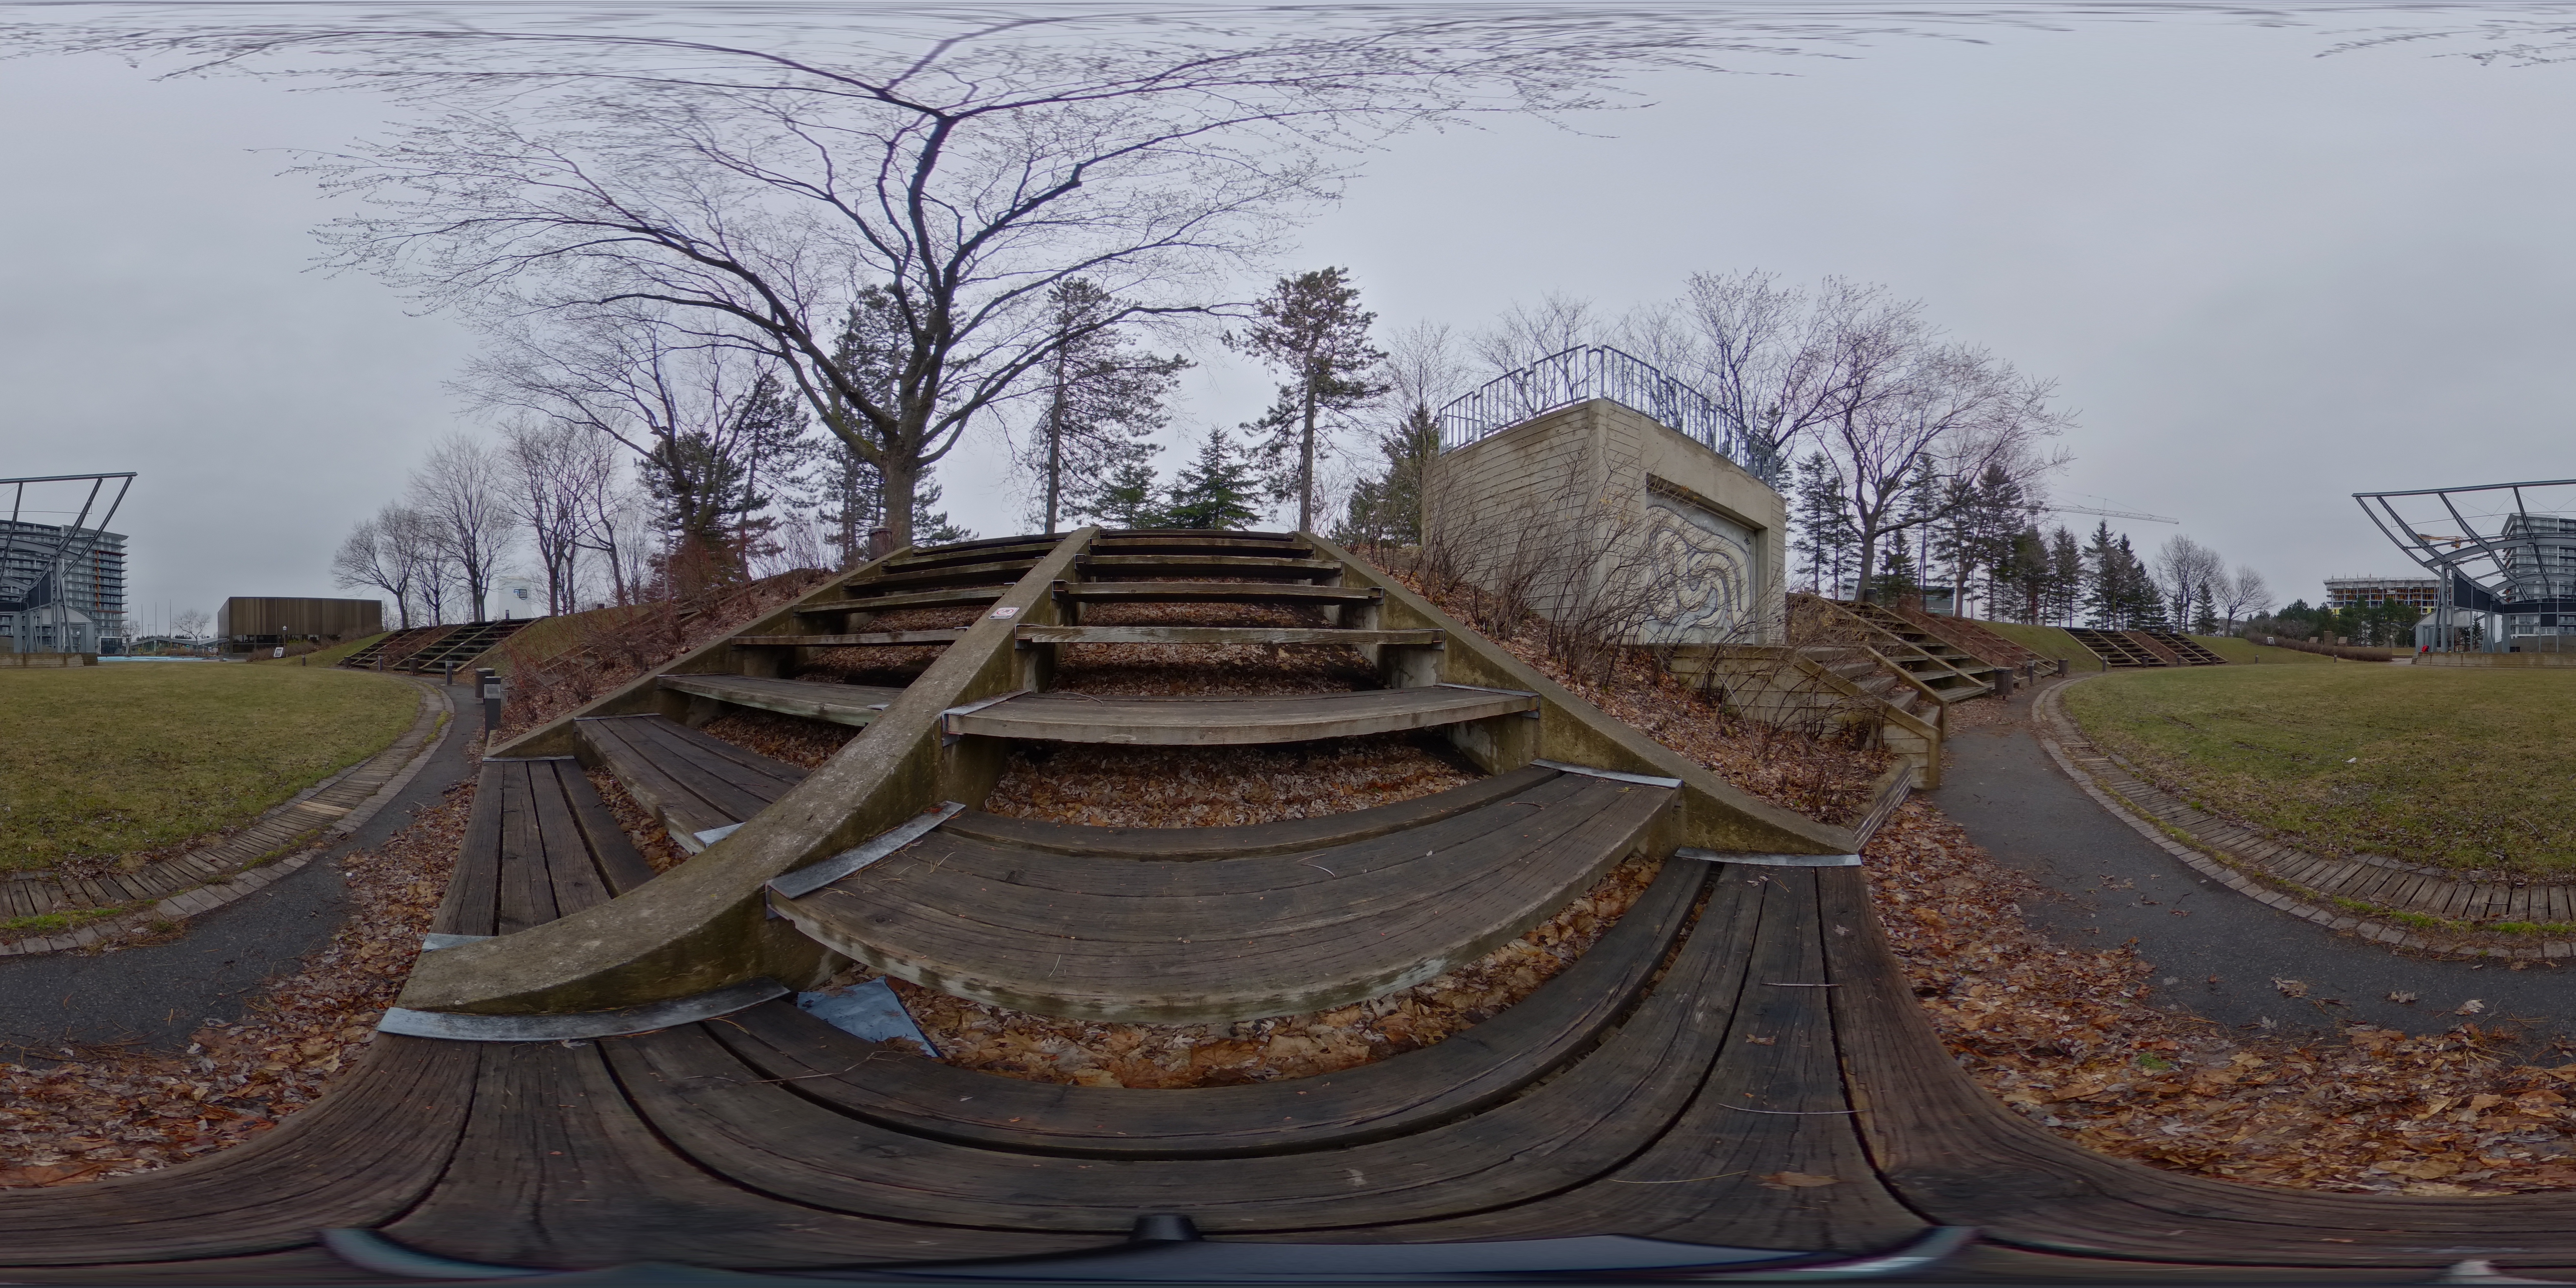
\includegraphics[width=0.9\textwidth, keepaspectratio]{02/mapping_latlong_photo.jpg}
            \caption{Equirectangular (latlong) mapping example}
    \end{subfigure}%
    \hfill
    \begin{subfigure}[t]{0.5\textwidth}
            \centering
            \includegraphics[width=0.9\textwidth, keepaspectratio]{02/mapping_latlong.jpg}
            \caption{Equirectangular distortion visualization}\label{fig:latlong-intro}
    \end{subfigure}
    \hfill
    \caption{Common mappings for 360\degree images}\label{fig:common_mappings}
  \end{figure}
  
\subsection{Optical Flow} \label{subsec:optical_flow}
Optical flow describes the displacement of specific points between two images. It is generally used on consecutive frames of video sequences, for example for semantic segmentation, structure-from-motion, data compression or other applications where information about movement between images is required. To illustrate, Figure~\ref{fig:of_example_bike} shows two consecutive frames of a video sequence. On a high level, an optical flow algorithm should recognize that the pixels representing the bicyclist are moving towards the bottom left of the image, and the pixels representing the background are moving to the right (because the camera is panning slightly to the left).

There are two types of optical flow: Sparse optical flow and dense optical flow. Sparse optical flow algorithms calculate the motion of several select points that can be either chosen manually, or by some kind of automatic selection (e.g. based on features). This type of optical flow can be used to track only specific objects in a scene (e.g. the direction and relative velocity of a certain car in traffic).

Dense optical flow algorithms compute the motion of \emph{each pixel} between two images, instead of single points. This can be used for more general object tracking (e.g. direction and relative velocity of complete surroundings in traffic), to estimate 3D geometry (in structure-from-motion algorithms), or to identify static sections of the image for video compression \cite{of-survey}. Dense optical flow can also be used for image synthesis, such as in Richardt et al's Megastereo \cite{megastereo} described in Section~\ref{subsec:megastereo}, which is also the basis of the flow-based interpolation presented in this thesis.

There are a number of optical flow algorithms, ranging from methods using parametrization, or regularization \cite{of-survey}, to methods relying on Deep Learning \cite{of-deep}. Although these algorithms differ greatly in approach, they have in common the type of result, which is a vector field. For dense optical flow, this vector field contains a vector for each pixel, describing the displacement of this pixel between the input images. Sparse optical flow only contains a vector for each pre-chosen point, not for every pixel.

Figure~\ref{fig:of_vis} shows two different visualizations of the vector field calculated by the dense optical flow algorithm by Farneb\"ack \cite{farneback} between the frames in Figure~\ref{fig:of_example_bike}. Figure~\ref{fig:of_vis}a is a color-based visualization: the hue encodes the vector direction, the saturation encodes the vector length for each pixel. Using this visualization, it is possible to roughly distinguish two separately moving areas of the image, which could be used for semantic segmentation. Figure~\ref{fig:of_vis}b shows the pixel displacements with vectors: the origin of the vector is shown by a point and the direction and length of the vector are represented by a line.

These visualizations can help in understanding if and how well an optical flow algorithm is working. Although there are a large number of different algorithms, most of them still struggle with common issues such as occlusions, too-large displacements and intensity changes \cite{of-survey}. Occlusions are problematic, since the displacements between two images may reveal or cover image areas that, as a result, have no correspondence in the previous image. This problem is exacerbated when displacements are very large (e.g. due to fast-moving objects). Large displacements are also problematic by and of themselves, as most algorithms are not designed to handle them. How these limitations affect the use of optical flow for image synthesis will be explored in Chapters~\ref{chap:implementation} and \ref{chap:evaluation}.

\begin{figure}
\centering
    \begin{subfigure}[t]{0.5\textwidth}            
            \centering
            \includegraphics[width=0.9\textwidth, keepaspectratio]{02/of_example1.jpg}
            \caption{Frame 1}
    \end{subfigure}%
     %add desired spacing between images, e. g. ~, \quad, \qquad etc.
      %(or a blank line to force the subfigure onto a new line)
    \begin{subfigure}[t]{0.5\textwidth}
            \centering
            \includegraphics[width=0.9\textwidth, keepaspectratio]{02/of_example2.jpg}
            \caption{Frame 2}
    \end{subfigure}
    \caption[Optical flow example]{Example frames that optical flow is calculated on}\label{fig:of_example_bike}

    \quad
    \begin{subfigure}[t]{0.5\textwidth}            
            \centering
            \includegraphics[width=0.9\textwidth, keepaspectratio]{02/of_vis1.jpg}
            \caption{Visualization of optical flow with color: the hue encodes the vector direction, the saturation encodes the vector length for each pixel.}
    \end{subfigure}%
     %add desired spacing between images, e. g. ~, \quad, \qquad etc.
      %(or a blank line to force the subfigure onto a new line)
    \begin{subfigure}[t]{0.5\textwidth}
            \centering
            \includegraphics[width=0.9\textwidth, keepaspectratio]{02/of_vis2.jpg}
            \caption{Visualization of optical flow with vectors: the origin of the vector is shown by a small point (only a limited number of vectors are shown)}
    \end{subfigure}
    \caption[Optical flow visualizations]{Optical flow visualizations}\label{fig:of_vis}
\end{figure}

\section{Related Work}
Image-based Rendering (IBR) and viewpoint interpolation\footnotemark\ started gaining interest with the advent of virtual walkthroughs, for example for Apple's QuickTime\textsuperscript{\textregistered} VR, in order to save render time by generating views from images instead of using complex 3D scenes including textures, lights and complex geometric models \cite{quicktime}.
Chen and Zhang, in their survey on image-based rendering \cite{survey2004}, use the terms \emph{source description} and \emph{appearance description} to compare these basic rendering techniques: ``Traditional'' rendering techniques use \emph{source description}, i.e. the scene is described by the objects within it, their positions and properties. On the other hand, IBR techniques try to achieve the same goal through \emph{appearance description}. Vision itself has little to do with 3D geometry; it is the processing of a dense set of light rays by the brain which are ``captured'' by the eye. This process can also be performed by a capture device like a camera. So, instead of trying to describe the scene through the objects it contains, IBR rendering techniques try to model the \emph{light rays} that reach the viewer. 

\footnotetext{There seems to be no explicit difference between ``image-based rendering'', ``viewpoint interpolation'' and ``viewpoint synthesis'' in literature, so they will be used interchangeably in this thesis, although ``interpolation'' is favored for more simple blending techniques, and ``synthesis'' is used to describe more complex algorithms.}

While the differentiation between source description and appearance description is helpful in understanding the basic differences between image-based and traditional rendering, many image-based rendering methods also utilize some form of source description, predominantly in the form of 3D geometry. In different survey on image-based rendering techniques, Kang and Shum \cite{survey2000} classify IBR rendering techniques on a continuum, which ranges from techniques using no geometry, to techniques using implicit geometry (i.e. feature correspondences), to techniques using explicit geometry (see Figure~\ref{fig:survey_categorization}).

\begin{figure}
		\centering
		\includegraphics[width=\textwidth]{02/shum_kang_survey.png}
    \caption[Categorization of IBR techniques from \cite{survey2000}]{Categorization of IBR techniques with representative members, taken from Kang and Shums ``A Review of Image-based Rendering Techniques''\cite{survey2000}}
		\label{fig:survey_categorization}
\end{figure}

The algorithm presented in this thesis is a combination of two different approaches: the first step uses no geometry whatsoever, and the second step uses feature correspondences to correct some problems that arise in the first step. This differentiation guides the related work presented here: The first section presents synthesis approaches using no geometry, and the second section presents approaches using implicit geometry or feature correspondences.
%Approaches using 360\degree images are preferred, but since these are less common than those using planar images, 
%Most research in the area of image synthesis is focused on planar images, but some 360\degree approaches can also be found.

%A theoretical model for \emph{appearance description} was developed by Adelson et al.\ \cite{Adelson91}: the \emph{plenoptic function} (Equation~\ref{eq:plenoptic}). The plenoptic function is a 7D function that describes the observable light at every point in space $V_x$, $V_y$, $V_z$, from every direction $\theta$, $\varphi$, at every wavelength $\lambda$, at every possible point in time $t$.

%\begin{equation}
%  \label{eq:plenoptic}
%  P = P(\theta, \varphi, \lambda, t, V_x, V_y, V_z)
%\end{equation}

%In practice, it is unfeasible, if not impossible, to cover all dimensions of this function, as this would require a capture device at every location, at every point in time, capturing light rays coming from every direction. However, by making assumptions, IBR techniques try to reconstruct simplified versions of the plenoptic function. Depending on which assumptions are made and how the surroundings are sampled, varying requirements are met and different results are achieved.

%Many of these approaches however, do use some geometry information in order to recalculate image points. The scene geometry is hereby either meticulously recorded at the time of the image capture, as with Kanade et al's 3D Dome \cite{geometry97}, or inferred from the image data alone, 

%The approach presented in this thesis is \emph{pixel-based}, i.e. using no geometry information, so the following section will first outline research aiming to synthesize viewpoints with the use of little to no geometry. Since the majority of pixel-based rendering research uses planar images, the second part will focus on research using 360\degree images, including approaches using geometry.

%\begin{itemize}
%  \item type of warping: uv mapping, warping based on triangulation and homography
%  \item image representation: cube, planar, sphere
%  \item constraints? color / angle / \ldots
%  \item geometry? sparse, dense, none
%  \item correspondences needed? sparse, dense, none
%  \item type of input: planar, 360, 180 pano
%  \item type of output: planar, 360, 180 pano
%\end{itemize}

\subsection{Image Synthesis with no Geometry}
\ldots light field rendering \cite{lightfield}

\begin{itemize}
  \item other approaches, such as light field approaches or neural network approaches
\end{itemize}

\subsubsection{``A Simple Method for Light Field Resampling'' \cite{simple_poster}}
Kawai \cite{simple_poster} approaches the problem of synthesizing new images with two degrees of freedom without using 3D geometry. Their basic setup is to capture four 360\degree images at each corner of a rectangular area and use resampling to synthesize a new image anywhere within this area.

The resampling is done by inserting a virtual sphere centered at the synthesized viewpoint representing a projection screen on which to project rays from the captured viewpoints. The locations of the captured viewpoints are known, so the outbound rays of these viewpoints can be calculated by using the image-to-world coordinate conversion from the equirectangular representation. The intersections of these captured rays with the virtual sphere are calculated and the corresponding pixel values used. The projection screen where no rays have intersected are approximated by repeating the reprojection with different resolutions.

In cases where several rays share an intersection, they use a rating based on the inner product of the ray direction and the viewing direction and use the ray with the smallest score. As an alternative, they suggest prioritizing one specific captured viewpoint over the others to completely avoid ghosting artefacts.

\subsubsection{``On the Use of Ray-tracing for Viewpoint Interpolation in Panoramic Imagery'' \cite{raytracing}}
%correspondences needed: none, geometry: none/dense, constraints: color-constraint, image rep: cube, type of warping: pixel blending
Shi et al.\ \cite{raytracing} examine how ray tracing can be used to calculate arbitrary new viewpoints based on knowledge of relative positions between the viewpoints which are stored as cube maps. For every pixel in the target image, a ray is cast into the scene. In order to find the correct value of that point, they use a color consistency constraint, which determines whether the pixel values of the reference images are similar. The assumption is that if the colors differ, the rays must not be intersecting the same point.

In order to calculate an intersection with the scene, they propose two different methods: A brute-force depth search using no scene geometry which searches along all of the captured rays until the pixel values are similar enough to fulfill their color constraint requirements, or a guided depth search using sparse 3D reconstruction.

To evaluate their method, they use a set of captured input images with a maximum distance of one meter, from which they remove one to use as ground truth. They evaluate the algorithm by describing the artefacts in the results and compare the brute-force with the guided depth search.

\subsubsection{``Unconstrained Segue Navigation for an Immersive Virtual Reality Experience'' \cite{segue}}
Herath et al.\ \cite{segue} propose a system that enables casual users to capture their surroundings with a smartphone in a grid and then navigate that environment with two degrees of freedom. In order to interpolate between two captured 360\degree images, they differentiate between faces that are parallel to the axis of movement and faces that are perpendicular to the axis of movement. For faces that are parallel, they stitch the faces of two adjacent viewpoints together and interpolate by using a sliding window. For faces that are perpendicular, they calculate a homography between the faces of two adjacent viewpoints and morph the image accordingly. To interpolate any image within a rectangular area bounded by four captured viewpoints, they recursively interpolate intermediary viewpoints until they reach the desired position.

Although they do not mention the dimensions of possible scenes, it must be assumed that the scenes are very large and objects very distant from the camera, since calculating a homography would not work given large perspective shifts.

%capture of scene in a grid
%1DoF interpolation:
%faces that are perpendicular \ar zoom (calculate homography between four corners and warp)
%faces that are parallel \ar stitch face from image 1 and two and slide window across depending on the distance travelled
%2DoF interpolation:
%extend for arbitrary points by using intermediate images
%not mentioned, but perspective shifts will not work at all \ar presumably only outdoor scenes with a large distance to the camera

\subsection{Image Synthesis with Implicit Geometry}
Leveraging image correspondences for synthesis has been a popular method almost since the beginning of viewpoint synthesis. Chen and Williams \cite{apple} were one of the first to use ``the morphing method'' that simultaneously blends the shape and texture of two images using image correspondences. A comparable method, based on optical flow, is used by Richardt et al.\ \cite{megastereo} for planar images.

Adaping planar algorithms (e.g. optical flow, structure-from-motion) for 360\degree images is a common challenge in 360\degree image synthesis. Kolhatkar et al.\ \cite{360flowblending} and Huang et al.\ \cite{6dof} solve this problem by extending the faces of the cube maps to account for pixels moving across borders. \cite{360flowblending} then use optical flow for interpolation between two images, whereas \cite{6dof} estimates the scene geometry with an SfM algorithm to extend monoscopic 360\degree videos to stereo. Zhao et al.\ \cite{cube2video} propose a method for adapting sparse correspondence matching for the spherical domain, circumventing the need to use an extended cube map.

Morphing the images to create a new viewpoint can be done with pixel-based blending \cite{megastereo}, \cite{360flowblending} or by triangulating the image and calculating homographies between the triangles \cite{6dof}, \cite{cube2video}.

%, and \cite{360flowblending} for 360\degree images, whose approaches are very similar to the flow-based blending step presented in this thesis.

%- triangulation based on correspondences + homographical morphing

The flow-based blending approach in this thesis builds on the approaches of \cite{megastereo} and \cite{360flowblending}, which are presented in more detail in the following sections.

\subsubsection{``Real-Time Virtual Viewpoint Generation on the GPU for Scene Navigation'' \cite{360flowblending}}
Kolhatkar and Lagani\`ere \cite{360flowblending} propose a method for smoothly interpolating between pairs of 360\degree images. Their approach leverages the optical flow calculated between 
Their approach is similar to the approach in Megastereo, where optical flow between the images is used to incrementally morph the two images. Since they use 360\degree images, they extend the cube map representation to account for points moving across edges, which is the method that is used in this thesis, as well. To reduce artefacts in the obtained optical flow, they perform a matching and smoothing step. They then implement their algorithm on the GPU, which allows them to interpolate between images in real-time. As to the maximum distances that are possible for interpolation, no definitive values are given, rather, ``reasonable'' distances are quoted.


\subsubsection{``Megastereo: Constructing High-Resolution Stereo Panoramas'' \cite{megastereo} \label{subsec:megastereo}}
%correspondences needed: dense, geometry: none, constraints: angle?, image rep: planar, type of warping: none, because planar
Richardt et al.\ \cite{megastereo} present an approach to combine planar images captured casually on a radius to create a panoramic image that is viewable in stereo in high resolution. In place of scene geometry, they use a cylindrical imaging surface that is concentric to the capture center. For each eye at a given viewing orientation, they project a ray into the scene (Figure~\ref{fig:megastereo}a) and calculate the deviation angle $\alpha$ between the desired ray and the nearest captured rays (Figure~\ref{fig:megastereo}b). 

\begin{figure}[]
\centering
\includegraphics[width=1\textwidth, keepaspectratio]{02/megastereo-figure.png}
\caption[Flow-based blending in Megastereo \cite{megastereo}]{(a) Illustration of rays required for creating a stereoscopic panorama and (b) deviation angles $\alpha$. (c) Duplication and truncation artefacts caused by the aliasing. (d) Flow-based upsampling to synthesize required rays. \emph{Adapted from \cite{megastereo}}}
\label{fig:megastereo}
\end{figure}

Linearly blending the rays of the two closest captures would lead to artefacts due to the difference between the real geometry and the cylindrical surface (Figure~\ref{fig:megastereo}c), and using a nearest-neighbor technique results in discontinuities. Instead, they propose a ``flow-based blending'' technique: For each ray of the final image that is not a captured ray (deviation angle 0), a new ray is synthesized using optical flow. The vertical image strip captured by the synthesized ray is interpolated by taking the two closest viewpoints $I_K$ and $I_L$ and interpolating $\widetilde{I_M}$ (Figure~\ref{fig:megastereo}d) using the optical flow vectors $F_{k\rightarrow l}$ and $F_{l\rightarrow k}$.  The corresponding strip is then taken from this new viewpoint which contains the matching ray.

%use a combination of image stitching and their own optical flow-based blending algorithm in order to account for . The goal is to synthesize stereoscopic viewpoints (an image for the left and right eye, each) from the set of captured monoscopic images. For the image strips for which a matching ray was not captured, they introduce a blending algorithm based on optical flow.

%After transforming the images so that they all have scene-independent orientation and minimal distortion, strips of the captured images are extracted for each ``eye'' based on the best matching image ray (Figure~\ref{fig:megastereo-figure}a and b). In cases where there is no perfect ray correspondence, the ray with the smallest deviation angle can be chosen, however, this can lead to artefacts as illustrated in Figure~\ref{fig:megastereo-figure}c. In order to mitigate these artefacts, Richardt et al.\ introduce a blending algorithm based on optical flow: 

%For Megastereo, there is no need to blend the complete images, instead, they restrict their calculations to the strips/pixels they need. For simplicity's sake, the process is described for a full image:
The interpolated image $\widetilde{I_M}$ at point $\eta$ between the images $I_K$ and $I_L$ is calculated by shifting $I_K$ by $\eta \cdot F_{k\rightarrow l}$ and by shifting $I_L$ by $(1 - \eta) \cdot F_{l\rightarrow k}$. The two shifted images are then blended linearly, using $\eta$ as the weight. Instead of calculating the entire image for each ray, only the necessary image areas are extracted and the interpolation is calculated pixel-wise.

According to the authors, their approach ``can handle angular resolutions from 1\degree to 4\degree, but even 8\degree produces agreeable results''. Although the approach is designed for planar images, the idea of leveraging deviation angles for  flow-blending approach is used 

%\subsubsection{6-DOF VR Videos with a Single 360-Camera}
%%correspondences needed: none, geometry: dense, constraints: none, image rep: cube, type of warping: triangulation
%Huang et al.\ \cite{6dof} propose a method to expand regular 360\degree video data into stereoscopic video data viewable with six degrees of freedom. Their approach is based on reconstructing the 3D scene and the camera path.
%
%This reconstruction is achieved by adapting well-established structure-from-motion (SfM) algorithms for 360\degree data by the same method as \cite{360flowblending}, by extending the cube map.
%Since SfM algorithms are designed for planar images with a limited field of view (FoV), the six separate faces of the cube map representation are used as input for the SfM algorithm. SfM algorithms work by tracking points across a series of images (e.g. frames), so for cube mappings, potential points moving across seams need to be accounted for. This is done by extending the field of view of each face so that regions around seams are represented on both sides of the seam. After the points are correctly tracked, the extended cube map is reduced back to its original format.

%The sparse scene geometry is inferred from the SfM data and then refined to a dense reconstruction using depth maps and triangulation. Finally, new viewpoints are synthesized by warping the current frame by using triangulation and warping the triangles (see Figure~\ref{fig:6dof}).
%Then, the sparse scene geometry and camera path are calculated by incrementation and interpolation. The sparse geometry is then refined to a dense reconstruction of the scene using depth maps and Delaunay Triangulation. Finally, new viewpoints are synthesized by warping the current frame. Their warping algorithm projects the dense 3D points to a unit sphere control mesh with icosahedral tesselation\footnote{Icosahedral tesselation of a sphere subdivides the surface of a sphere into triangles. Other terms for this type of sphere are Icosphere or Geodesic Polyhedron} for both the captured viewpoint and the desired viewpoint. Then the vertex motion between each pair of triangles is calculated and the image warped according to these motion vectors (see Figure~\ref{6dof-figure}). 

%\begin{figure}[]
%\centering
%\includegraphics[width=0.6\textwidth, keepaspectratio]{02/6dof-figure.jpg}
%\caption[Image warping from Huang et al. \cite{6dof}]{The warping field is computed by finding the movement between the projections of each 3D scene point in the reference and the synthesized frame. Then the warping field is used to map each pixel of the synthesized image to its corresponding pixel in the reference to look up its color information. \emph{Adapted from \cite{6dof}}}
%\label{fig:6dof}
%\end{figure}



    %\chapter{Proof of Concept Design and Implementation}
%\chapter{Pixel-based Synthesis of 360\degree Viewpoints}
%\chapter{Pixel-based Synthesis of 360\degree Viewpoints with 2DoF}
\chapter{Pixel-based Rendering of 360\degree Viewpoints with 2DoF}
\section{Approach}
%\begin{itemize}
%  \item most other approaches rely on either geometry or correspondences
%  \item usually some form of triangulation
%  \item use of sphere for ray tracing, then use texture lookup to find the pixel values
%  \item combination of reprojection ie warping with angle constraint and flow-based blending
%  \item first part relies on radius/scale, but no geometry, second part relies on image correspondences
%  \item ``view-dependent texture maps'' \ar environment map / viewpoint is chosen based on some kind of proximity to the synthesized view
%  \item pixel-based, in that each pixel is calculated separately, there are not image-area based constraints
%\end{itemize}

\subsection{Assumptions}
\begin{itemize}
  \item all images are oriented the same
  \item all images were captured on a plane parallel to the floor
  \item the positions of the captures are known
  \item the scale (radius) of the scene is known
  \item all synthesized viewpoints are located inside the scene boundaries
\end{itemize}

\subsection{Basic 2DoF Synthesis}
With these assumptions and using a basic model geometry with the same scale as the captured scene, it is already possible to synthesize new views of approximate to exact accuracy, depending on the scene. The process for basic 2 degree of freedom synthesis presented is a combination of texture-lookup through raytracing, and mosaicking by using a deviation angle constraint.

\subsubsection{Raytracing-based Texture Remapping}
The first step is to remap the texture (i.e. pixel values) of an existing viewpoint to a new viewpoint according to its position in the scene. Theoretically, any 360\degree viewpoint can be remapped to any other, since each 360\degree image captures each point in the scene. This is only theoretically the case, since resolution and occlusions in the scene will conceal some areas for some viewpoints whereas they are visible for others. However, at this point, this will be ignored and it will be assumed that each viewpoint image contains all the points of the scene albeit at different image coordinates and different sampling rates\footnote{Areas closer to the camera are captured with higher sampling rates than areas farther away.}. 

Furthermore, a 3D geometry is needed for calculating ray-scene intersections. Since the approach in this thesis does not capture or infer any real geometry, a model geometry is used that has approximately the same scale as the scene that was captured. The model geometry used is a sphere, as this is a simple, very general geometry to represent a variety of different scenes. The radius of the sphere is chosen so that the sphere contains all possible points in the scene, for which the scale of the scene needs to be known. Under these assumptions, it is possible to remap the image at one viewpoint to a different position.

% This is visualized in Figure~\ref{fig:reflected_rays} a: Each point P of the scene reflects light rays in all directions. These light rays are captured at different viewpoints and are discretized into pixels in the image taken at that viewpoint. As a result, the pixels representing point P are present in the images captured at each viewpoint. This means that when synthesizing a new viewpoint S, the pixels representing point P can theoretically be retrieved from any of the images at the captured viewpoints (Figure~\ref{fig:reflected_rays} b).

In order to do this, several steps of raytracing are necessary, which are visualized in Figure~\ref{fig:raytracing}. Figure~\ref{fig:raytracing} a shows how a camera at a specific viewpoint captures the light rays reflected from the objects in the scene. The captured pixel values are visualized on a circle around the center of projection of the camera (for simplicity's sake, only one row of pixels is shown). Once the viewoints have been captured (there is only one in this example), a new viewpoint is ready to be synthesized. The model geometry is visualized as a circle in Figure~\ref{fig:raytracing} b, with the new viewpoint to be synthesized represented by a dotted circle around a center of projection. For each pixel of the synthesized image, a ray is projected into the scene (Figure~\ref{fig:raytracing} c) and its intersection with the scene is calculated. Then, the ray from the center of projection of the captured viewpoint to the scene intersection is calculated and the pixel value at that position in world coordinates is retrieved (Figure~\ref{fig:raytracing} e) and copied back to the new viewpoint (Figure~\ref{fig:raytracing} f). This way, the pixel values (i.e. texture) of a captured viewpoint are remapped to the new viewpoint (Figure~\ref{fig:raytracing} g). Figure~\ref{fig:raytracing} compares the remapped values to the actual scene. It is immediately visible that

\begin{figure}
\centering
    \hfill
    \begin{subfigure}[t]{0.3\textwidth}            
            \centering
            \includegraphics[width=0.9\textwidth]{03/raytracing01.png}
            \caption{The real scene viewed from above: The camera captures light rays reflecting from objects}
    \end{subfigure}%
    \hfill
     %add desired spacing between images, e. g. ~, \quad, \qquad etc.
      %(or a blank line to force the subfigure onto a new line)
    \begin{subfigure}[t]{0.3\textwidth}
            \centering
            \includegraphics[width=0.9\textwidth]{03/raytracing02.png}
            \caption{A new viewpoint to be synthesized using the model geometry (sphere)}
    \end{subfigure}
    \hfill
    \hfill

    \hfill
    \begin{subfigure}[t]{0.3\textwidth}            
            \centering
            \includegraphics[width=0.9\textwidth]{03/raytracing03.png}
            \caption{A ray for each pixel in the synthesized viewpoint is traced to its intersection with the model}
    \end{subfigure}%
    \hfill
    \begin{subfigure}[t]{0.3\textwidth}
            \centering
            \includegraphics[width=0.9\textwidth]{03/raytracing04.png}
            \caption{For each ray, a texture lookup is performed}
    \end{subfigure}
    \hfill
    \begin{subfigure}[t]{0.3\textwidth}
            \centering
            \includegraphics[width=0.9\textwidth]{03/raytracing05.png}
            \caption{From the ray-model intersection, a second ray is traced to the center of projection of the captured viewpoint and the pixel value is looked up}
    \end{subfigure}
    \hfill

    \hfill
    \begin{subfigure}[t]{0.3\textwidth}            
            \centering
            \includegraphics[width=0.9\textwidth]{03/raytracing06.png}
            \caption{The pixel value is copied back to the new viewpoint}
    \end{subfigure}%
    \hfill
    \begin{subfigure}[t]{0.3\textwidth}
            \centering
            \includegraphics[width=0.9\textwidth]{03/raytracing07.png}
            \caption{This process is repeated for all pixels}
    \end{subfigure}
    \hfill
    \begin{subfigure}[t]{0.3\textwidth}
            \centering
            \includegraphics[width=0.9\textwidth]{03/raytracing08.png}
            \caption{The resulting texture mapping from the captured viewpoint to the model geometry in comparison with the original scene}
    \end{subfigure}
    \hfill
    \caption[Process of texture lookup through raytracing]{Process of texture lookup through raytracing}\label{fig:raytracing}
\end{figure}


\paragraph{Ray-sphere intersection}
The vectors representing these rays can be easily derived from the \emph{world coordinates} of the image (see~Section~\ref{fundamentals_360}).

The intersections of these rays with the model geometry can be calculated analytically: The sphere representing the scene can be represented implicitly by Equation~\ref{eq:rsi_spherefull}. The set of points P defined by this equation make up the surface of the sphere (Equation~\ref{eq:rsi_sphereP}). 
The equation describing any point on the ray can be expressed by Equation~\ref{eq:rsi_point}, where $O$ is the origin of the ray, which is the center of projection of the new viewpoint, $t$ is the length of the ray and $D$ is a unit vector describing the direction. 

\begin{align}
  x^2 + y^2 + z^2 - R^2 = 0&\label{eq:rsi_spherefull}\\ 
  P^2 - R^2 = 0&\label{eq:rsi_sphereP}
\end{align} 
\begin{align}
  P = O + tD& \label{eq:rsi_point}
\end{align} 

The point $P$ in Equation~\ref{eq:rsi_sphereP} can be substituted with the equation of the any point on the ray which yields Equation~\ref{eq:rsi_sub}. This equation can be developed into Equation~\ref{eq:rsi_quad}, which is a quadratic function with $a = D^2$, $b = 2OD$, $c = O^2-R^2$ (Equation~\ref{eq:quadf}).

\begin{align}
  |O + tD|^2 - R^2 &= 0  \label{eq:rsi_sub}\\
  D^2 t^2 + 2ODt + O^2 - R^2 &= 0 \label{eq:rsi_quad}
\end{align}

\begin{align}
  a = D^2, b = 2OD, c = O^2-R^2 \\
  f(t) = at^2 + bt + c \label{eq:quadf}\\
  t = \frac{-b \pm \sqrt{b^2 - 4ac}}{2a} \label{eq:solvequadf}
\end{align}

This equation can then be solved for t. Since the radius of the sphere is chosen so that it contains the complete scene and no viewpoints are synthesized outside of the scene, the quadratic function will always have two solutions (i.e. two intersections): one for which the vector length $t$ is negative, and one for which the vector length is positive. The positive value is used to find the intersection in question.


%\begin{figure}[]
%\centering
%\includegraphics[width=1\textwidth]{03/incoming_lightrays.png}
%\caption[Light rays reflected from a point in the scene]{The reflected light rays from each point in the scene are captured by each 360\degree viewpoint}
%\label{fig:reflected_rays}
%\end{figure}

%\begin{itemize}
%    \item all viewpoints more or less capture complete surroundings from different perspectives \ar each point from an input viewoint will be somewhere on the synthesized viewpoint
%    \item find corresponding points with the output viewpoint for each input viewpoint (\emph{``where would point P (seen in viewpoint A) be in the synthesized viewpoint S''})
%    \item to determine which viewpoints to use for which output image areas, use weighting function $W(viewpoint)$ that is dependent on specific properties of the input viewpoint (e.g. euclidean distance of locations)
%    \item in order to do all this, need scene model which is a sphere since we have no geometry information
%\end{itemize}

%The main difference between 1DoF and 2/3DoF synthesis is that in 1DoF interpolation, the choice of viewpoints is trivial, as there are only two by definition. In 2/3DoF synthesis, the idea is to have an unlimited number of viewpoints as input (for 2DoF synthesis, these viewpoints must all be on a plane). Since all the images are 360\degree images, each one theoretically captures the complete surroundings. This means that every existing point should be present somewhere in each image (ignoring occlusions at the moment).
%The basic idea of the 2/3DoF algorithm is to find the image areas from the set of existing viewpoints that are the ``most fitting'' for the synthesized viewpoint and transform these areas to approximate where they would be in the synthesized image. This means that a metric is necessary that measures how ``fitting'' a specific pixel of a viewpoint image is. Also, a reprojection needs to be found that transforms the ``fitting'' image areas to the appropriate image coordinates for the synthesized viewpoint.
%\missingfigure{point correspondences and reprojection intro}


\subsubsection{Deviation angle constraint}
- different sections of different viewpoints may be more appropriate in terms of accuracy
- use deviation angle as constraint (other possibilities are also possible, such as a combination of deviation angle and distance)
- calculate deviation angle and blend the best 2 based on a blending function (inverse sigmoid)

%In order to find the ``most fitting'' image area from all of the viewpoint images, there first needs to be a metric that measures how ``fitting'' an image area is. 

%One example is the euclidean distance of the viewpoint locations in space. This would mean that for each pixel, the corresponding pixel of the \emph{nearest viewpoint} would be used. This is the simplest approach, and would simply return the nearest neighbor. 

\subsection{2DoF Synthesis using Flow-based Blending}
- using only basic 2DoF synthesis works fairly well as long as the actual geometry of the scene corresponds more or less to the model geometry (sphere)
- ghosting/aliasing problems as soon as objects are closer or farther than the sphere radius
- use flow-based blending from Megastereo to improve this

%The simplest type of synthesis in the scope of this thesis is the creation of a new viewpoint that lies exactly on a line between two existing viewpoints. Assuming that the existing viewpoints are facing the same direction, the line describes a transformation with one degree of freedom, i.e. movement along the line. A solution to a similar problem has already been published by Richardt et al. in ``Megastereo'' \cite{megastereo} which introduces an approach using optical flow in order to reduce ghosting artefacts in planar images. The following section shows how the problem of 1D interpolation for 360\degree images can be reduced to the problem solved in Megastereo.

\subsubsection{Flow-based Blending in Megastereo}
%Megastereo aims to generate high-resolution stereo panoramas by combining images captured on a circle. Their approach is to combine corresponding strips of the captured images and to create a view for each eye (see section \ref{megastereo}). In order to mitigate artefacts such as ghosting, they use ``flow-based blending'' to combine two images A and B. This consists of using the optical flow vectors $F_{A\rightarrow B}$ and their inverse $F_{B\rightarrow A}$. To get the interpolated image at position $\alpha$ between image A and B, first, image A is shifted by $\alpha \cdot F_{A\to B}$ and image B is shifted by $(1 - \alpha) \cdot F_{A\to B}$, yielding $I_A$ and $I_B$, respectively. Then, $I_A$ is multiplied by $(1-\alpha)$ and $I_B$ by $\alpha$ and these pixel values are added together to give the resulting interpolation. This is described by the following function, in which each pixel at position x is defined by: 
%\begin{align}
%S(x) = (1-\alpha ) \cdot I_A( x + \alpha \cdot F_{A\to B}(x) \\
%     + \alpha \cdot I_B( x + (1-\alpha) \cdot F_{B\to A}(x))
%\end{align}

\subsubsection{Reducing 360\degree Interpolation to Planar Interpolation}

A 360\degree image can be projected in several ways, as described in Section \ref{projections}. The output of these projections is a planar image, meaning that flow-based blending could be applied directly. However, this would not lead to optimal results for several reasons: Most projections distort the image in some areas, which would result in distorted optical flow values. Furthermore, in order to make planar viewing possible, the 360\degree image must be ``unfolded'' along some seam. When calculating optical flow, points that move across the seam will not be tracked, even though they do not move out of the image space, as would happen in a regular image.
\missingfigure{points moving across edge in regular vs 360\degree image}

Of the existing projections, only two really come into consideration for this problem: the equirectangular representation and the cubemap representation. Spherical representations are impractical, as aligning seams is not feasible. The equirectangular representation has fewer seams to handle, but also distorts the image greatly around the poles. The cubemap representation hardly distorts the image at all, but contains a number of seams. In this case, the distortion is more difficult to deal with, since the effects on the optical flow algorithm are unclear. Handling seams is more straightforward, which is why the cubemap representation was chosen for 1D interpolation.

In order to handle points moving across seams, the optical flow algorithm must be able to read data \emph{across the seams}. For example, when calculating optical flow on the ``front'' face, data from the ``top'', ``left'', ``right'' and ``bottom'' faces is required. Intuitively, one might just assemble these faces in a plus shape, with the ``front'' face at the center. However, this is a fallacy, since the cubemap projection uses a different virtual camera for each face, which means that linearity is not preserved for points moving across seams.

\missingfigure{cubemap with point moving across seam}

To solve this problem, the ``extended cube map'' is introduced, which was also used by Huang et. al. \cite{6dof}. Instead of projecting a field of view of 90\degree for each camera, which covers 360\degree of the image, the extended cube map uses a larger field of view for each camera. As a result, the areas of the image that are split by a seam are represented twice: Once on each face that is adjacent to the seam. This way, when calculating optical flow on each face separately, points that move across where the seam would be in a regular cube map remain on the face with the corresponding projection. 

Naturally, this method is limited by the field of view used by the virtual cameras. If the maximum displacement is larger than the face extension, the extended cube map will not be sufficient, which will result in black edges on the faces. Also, the larger the field of view, the more the image will be distorted towards the edges of a face, which may lead to distorted optical flow results. This means that displacement between two images is limited. However, the displacement that is trackable by optical flow algorithms is also limited. The effect of these limitations will be explored in section \ref{evaluation1D}.

Using the extended cube map, it is possible to process each face separately, meaning that the 360\degree 1DoF interpolation has been reduced to planar images. At the end of the interpolation step, the extended cube map must be clipped back to the original cube map size.
\missingfigure{1D interpolation process diagram}

%further points to include
%- inverting flow is non-trivial

\section{Implementation}

\subsubsection{Preprocessing and CaptureSet}
\begin{itemize}
  \item rotate all images so that they all have the same orientation
  \item center point cloud
  \item find appropriate sphere radius
  \item make access to location and image data of a viewpoint contained in a set easy and intuitive
\end{itemize}

\subsubsection{Interpolation}
\begin{itemize}
  \item ray and scene intersection
  \item viewpoint reprojection
  \item deviation angle calculation
  \item weighting function
\end{itemize}

\subsection{Debugging and Verification}
\begin{itemize}
  \item in order to verify correct results and check for bugs, use of the ``checkersphere'' in which the scene model exactly matches the scene \ar reprojection will yield exact results (excluding resolution)
  \item explain why it will yield correct results and why the resolution is not perfect
\end{itemize}

\subsection{Implementation challenges}
``one on each side''
\begin{itemize}
  \item define ``on either side'' for angles: split the circle in two 180\degree halves; one is positive, the other is negative
  \item selection of a viewpoint ``on either side'' \ar what if the viewpoint on one side has a very large deviation angle or does not exist?
  \item can it not exist if we are looking at the convex hull? Yes, if the point is exctly on the border
  \item possible solution: if none is found, use only one side
  \item what to do with zero degree difference? \ar only use zero, not the other (should be solved by the function that defines the 1D interpolation position)
\end{itemize}
using only 2D data
\begin{itemize}
  \item ``left and right'' only possible in 2D (can use signed angles)
  \item in 3D, finding viewpoint on ``either side'' becomes a lot more complex
  \item reducing viewpoints to 2D is simple, but scene model is still in 3D. simplifying scene model to 2D as well
\end{itemize}

errors that are unrelated to the algorithm:
\begin{itemize}
  \item slight displacement due to ExtendedCubeMap
  \item black edges due to latlong-cube conversion
  \item these need to be taken into account (normalized out)
  \item only an issue for flow-based because flow-based uses conversion, whereas regular does not
\end{itemize}

\subsection{Performance}

    \chapter{Evaluation and Results} \label{chap:evaluation}


\begin{verbatim}
- no publicly available benchmarks for 360\degree image synthesis / image based rendering available for comparison with other methods
- scope: basic evaluation of mathematically measurable values (no human perception)
- create virtual datasets to test the limits of the method
- capture real datasets to perform a proof of concept

- these datasets could be used in the future to compare different algorithms
- benchmark used will be nearest neighbor (naive algorithm)
\end{verbatim}

\section{Evaluation Methodology}
In order to evaluate the effect of different parameters on the 2DoF synthesis algorithm developed in \ar scenarios, whether the
The evaluation process of each scenario is divided into four phases: scenario definition, where the parameters to test in the scenario are selected, synthesis, where the synthesized images are calculated using the 2DoF synthesis presented in chapter~\ref{chap:implementation}, error calculation, where the accuracy of the synthesized images is measured, and result analysis, where the the cause and effect of the parameters is examined. 

\begin{figure}
		\centering
		\includegraphics[width=\textwidth]{04/eval_methodology.png}
		\caption{Evaluation Methodology}
		\label{fig:eval-methodology}
\end{figure}

\subsubsection{Scenario Definition}
First, a scenario must be defined that illustrates the parameter that should be examined. This includes determining which of the parameters should be static, and which should be dynamic. There are two dynamic parameters at maximum, one to be examined, and one to increase the significance of the results. Adding more dynamic parameters at per scenario would allow for a more definitive evaluation, but is outside of the scope of this thesis.

The set of parameters (whether static or dynamic) contains the choice of scene in which to synthesize the images. The scene is defined by its captured viewpoints, metadata, and radius, which are all passed on to the synthesis step along with the other parameters defined for the scenario.

\subsubsection{Synthesis}
The synthesis step consists of two parts: the 2DoF synthesis presented in \ref{chap:implementation} using either flow-based blending or regular blending depending on the scenario parameters, and a baseline synthesis using a trivial algorithm. The results of the trivial algorithm serve as a baseline comparison to verify whether the developed 2DoF algorithm is an improvement to a naive approach. The trivial algorithm consists of simply selecting the nearest neighbor viewpoint based on euclidean distance. The input parameters are the same for both algorithms and both results are passed on to error calculation.

\subsubsection{Error Calculation}
In order to evaluate the synthesized images, it is necessary to define metrics with which to measure their accuracy. Since it is outside of the scope of this thesis to evaluate the quality of the results based on human perception, mathematical error metrics are used to compare each result to its ground truth image. Two different metrics are chosen based on different image features so that potential limitations of each metric can be compensated for by the other.

\paragraph{L1 error on RGB}
The first metric is the L1 error calculated on the ground truth and result images in RGB color space. This is a simple error metric that calculates the mean absolute difference of the RGB values and therefore indicates the mean accuracy of each pixel of the image. The RGB errors of each pixel are added together for the complete image and then divided by the number of pixels in the image. This results in an error value $e \in [0,3]$, since the maximum error per pixel is 3 for floating point RGB color values $\in [0,1]$.

The L1 error can also be visualized by calculating the absolute difference per pixel without averaging the values. Figure~\ref{fig:l1_example} shows an example visualization of the L1 error between two images. The visualization encodes areas of the image where there is a very large difference with a value closer to white and areas where there is no difference as black, which clearly shows where the problematic areas are in the image.

The L1 error is useful because it gives a rough estimation of how accurately each pixel is synthesized. The visualization indicates in which areas the synthesized image is inaccurate, which is helpful for classifying problems. However, a drawback of the L1 error is that it relies on color values, which means that images with large differences in pixel values will generally produce a higher error value than images with smaller differences in pixel values, even though the distortion and displacement is the same. \todo{maybe example with checkerboard?}

\begin{figure}
\centering
    \hfill
    \begin{subfigure}[t]{0.3\textwidth}
            \centering
            \includegraphics[width=0.9\textwidth]{04/l1_ex01.jpg}
            \caption{}
    \end{subfigure}%
    \hfill
    \begin{subfigure}[t]{0.3\textwidth}
            \centering
            \includegraphics[width=0.9\textwidth]{04/l1_ex02.jpg}
            \caption{}
    \end{subfigure}
    \hfill
    \begin{subfigure}[t]{0.3\textwidth}
            \centering
            \includegraphics[width=0.9\textwidth]{04/l1_ex03.jpg}
            \caption{L1 error visualization of (a) and (b)}
    \end{subfigure}%
    \hfill
    \hfill
  \caption[Example visualization of L1 RGB error]{Example visualization of L1 RGB error. The RGB error values have been intensified so that they are more visible.} \label{fig:l1_example}
\end{figure}

As in the case of optical flow calculation, some adjustment must be made to adapt this metric for 360\degree images. Since the equirectangular projection is not equal-area, the areas towards the poles would intrinsically have higher weighting, since RGB L1 is calculated per pixel. In order to avoid this problem, the cube map projection is used, since it does not significantly distort the image. The average value is then calculated using the six faces of the cube, omitting the black background.

\paragraph{SSIM error on Grayscale}
The other metric to complement the RGB L1 error uses the structural similarity index (SSIM) \cite{ssim}, which measures the \emph{similarity} between two images. Instead of comparing the images pixel by pixel, the SSIM uses the luminance, contrast and structure of the images for comparison. It compares these locally, i.e.\ it compares smaller areas instead of the image as a whole. As a result, it is possible that the SSIM does not register small displacements in the scene if the objects are not distorted. However, the additional comparison with the RGB L1 error should mitigate this potential problem.

The SSIM metric in general, and the implementation used in the evaluation\footnote{skimage.metrics.structural\_similarity \cite{skimage}} return a value $\in [-1, 1]$ with 1 signifying an extremely similar image and -1 signifying a very different image. In order to more easily compare it with the RGB L1 error, the SSIM value is converted to an error value $ e \in [0,1]$, with 0 signifying an identical image and 1 signifying a very different image.

The SSIM error is calculated on the grayscale image in cubemap representation. There is no need to use an RGB image, since it does not use the color values of an image. To avoid possible problems with distortion, the cubemap representation is again used.

\subsubsection{Result Analysis}
The number of parameters and synthesized viewpoints combined with the comparison to the baseline results and the use of two different error metrics results in a large number of error values. In order to analyse these effectively, it is necessary to create different visualizations that highlight different attributes of the results.

\paragraph{Distribution Comparison}
The analysis starts with a comparison of error value distribution. In order to compare all the error values of a scenario, they are plotted using a boxplot. The different parameter variations of the scenario are plotted on the y axis and the error distribution (i.e. the error values of all the synthesized viewpoints) are plotted on the x axis. This allows for a general evaluation of the effect of the parameters examined in the scenario.

\paragraph{Scene Analysis}
Based on the insights gained in the distribution comparison, several interesting cases are selected for closer analysis. These cases are then examined by putting the error values of the synthesized viewpoints in context with the scene surroundings by color coding the error values and assigning the colors to the positions in the scene (e.g. Figure~\ref{fig:posmap_example}). For comparisons between different visualizations, the same color mapping is used. This way, it is possible to estimate the effect of the scenario parameters in conjunction with the scene geometry, which can help with understanding the effect of the parameters on the result accuracy.

\begin{figure}
		\centering
		\includegraphics[width=0.3\textwidth]{04/posmap_example.jpg}
		\caption{Example of the Scene Analysis Visualization: The error values are mapped to colors, with dark red representing the worst and dark blue the best value.}
		\label{fig:posmap_example}
\end{figure}

\paragraph{Sample Inspection}
In order to further understand the effects of the parameters on specific positions, some of the synthesised viewpoints from the scene analysis are examined manually by comparing the synthesized image to the ground truth image. The manual examination may also reveal information that the error metrics are unable to extract.

\section{Evaluation of Limits using Virtual Scenes}

\subsection{Parameters}
internal vs external parameters
\begin{itemize}
  \item internal:
  \item viewpoint density
  \item distance of scene from model (checkersphere, square room, arbitrary room)
  \item flow-based blending vs deviation-angle-based blending
  \item external:
  \item number of samples/viewpoints used for interpolation \ar two vs all within semi-large radius (all would be very computation intensive)
  \item limit to certain scenarios so that the explored space stays manageable
\end{itemize}

parameters that are not examined (within the assumptions of the function)
\begin{itemize}
  \item choice of gt points \ar fixed
  \item \ar offset of synth point from the line between two points (this would measure the effect of th 2DoF approximation
  \item distance from captured point (in the scenes, the gt points are always the furthest possible distance from all other points)
  \item optical flow accuracy in relation to the scene size etc
\end{itemize}
limitations also here?

\subsubsection{Choice of Ground Truth Viewpoints and Captures}

\subsubsection{Selection of Input Viewpoints}

\subsubsection{Scene Distance from Model Sphere}
Checkersphere, square room, oblong room, (oblong room v2)

\subsection{Synthesizing Ground Truth Optical Flow}
 only makes sense to compare if flow algorithm works more or less correctly \ar narrows the parameter space for comparison
\begin{itemize}
  \item optical flow ground truth is impossible to get from real scenes
  \item however, virtual scenes contain all necessary information for retrieving ground truth for optical flow
  \item virtual camera rig that captures one image per ``side'' with a fov that corresponds to that used in the ExtendedCubeMap \ar extended flow cube
\end{itemize}

``correctness'' of optical flow interpolation is limited even with ``perfect'' optical flow:
\begin{itemize}
   \item points that are not visible because of perspective shift will not have a correspondence
   \item distortion due to wide fov may have an effect on the results
   \item even blender motion vectors are for frame to frame use, so it is possible, that large jumps do not work well because the blender algo can't handle it
\end{itemize}

\subsection{Results}
\subsubsection{Minimum vs Maximum Number of Input Viewpoints}
input selection and scenes are var, all others are fixed
\begin{verbatim}
Hypothesis: 2vps is better for flow-based, radius is better for regular.
flow based does not do well with image patches with different viewpoint indices
(extreme discontinuities)

Test: 
  -use the two simplest scenes with a medium number of viewpoints and synthesize using
only two vs all within the radius of 1/2*scene radius

Show: 
  - compare flow to flow and regular to regular
      --> we only want to know which is better for each blending method,
      not in comparison

Even if the hypothesis is not proven, or is not very distinct,
can still argue that >2 or >4 is computationally too costly for consideration

\end{verbatim}

\subsubsection{Viewpoint density effect on flow-based blending and regular blending}
density, blending var, others fixed
\begin{verbatim}
Hypothesis: higher density --> better results, but difference is larger for flow-based.
(optional: High density and 2vps may be better than 4)

Hypothesis II: the effect of higher density is more marked near walls and corners

Test:
  - use square room and test 2x2, 6x6, 10x10
  - compare flow with flow, reg with flow, and reg with reg -> 3 graphs

\end{verbatim}

\subsubsection{Flow-based blending vs regular depending on model-scene difference}
blending and scene var, others fixed
\begin{itemize}
  \item ``checkersphere'' in which the scene model exactly matches the scene
    \ar reprojection will yield exact results (excluding resolution)
  \item explain why it will yield correct results and why the resolution is not perfect
\end{itemize}
\begin{verbatim}
Hypothesis: the closer the scene is to the model, the better regular blending is.
the farther away, the worse it is and the better flow-based blending is

Test: compare the two with their respective better vp selection in the different scenes

\end{verbatim}


\section{Proof-of-Concept Evaluation of Real Scenes}

\section{Discussion}

\subsection{Limits}

limits of the evaluation:
\begin{itemize}
  \item interactions between the parameters are not closely examined \ar possible that some parameter affects another in an unexpected way
  \item objects are not clearly classified/measured, so no quantifiable evaluation possible
  \item positional and rotational knowledge may be calculable by sfm algos, but we don't know what kind of impact accuracy of the metadata will have, since we are hand-recording metadata meticulously
  \item pixel differences and ssim give no indication on human perception, so it is not possible to judge believability
  \item even though the results suggest it, cannot be sure that the metrics measured are significant/robust
  \item all gt points are exactly in the middle of input points (except 2x2) this has a definite effect on optical flow interpolation, especially between 2 viewpoints
  \item interactions between different parameters are not examined exhaustively, so no conclusive information
\end{itemize}

Assuming radius accuracy does in fact make a slight assumption about the scene geometry. Using only the deviation angle will lead to ``spots'' where the distance is fairly large but the angle is zero. 

\subsection{Future Work}
\begin{itemize}
  \item ``guess'' an optimal radius without using viewpoint locations e.g. outside
  \item find a good weight function that balances deviation angle and distance appropriately
  \item use methods like SLAM in order to be independent of actually recording metadata by hand
  \item undistort extended cubemap e.g. by using methods like \cite{fov} which can undistort images up to 120\degree
  \item extend to 3D \ar input viewpoints could improve flow-based blending for areas towards the poles
  \item parallelization and offloading to gpu
  \item improve choice of $\delta$
  \item human perception evaluation with user study
\end{itemize}


    \chapter{Conclusion}

The approach and implementation presented in this thesis laid the groundwork for a pixel-based 2-DoF synthesis using 1-DoF interpolation, which combines
straightforward, pixel-based reprojection using proxy geometry with flow-based interpolation in order to generate more accurate results.
The evaluation provided insights on the strengths and limitations of this approach, which can be used in the future in order to improve the proof-of-concept implementation.
On the basis of the approach developed in this thesis,
%real-time navigation of previously captured scenes with 2 DoF , which could be used to experience
casually captured environments could be experienced interactively, which could enhance a broad range of Virtual Reality applications.





    \appendix
    \chapter{Synthesized Images}\label{imgs}

\begin{figure}
		\centering
		\includegraphics[width=\textwidth]{04/inspection_example_K.jpg}
		\caption{Sample inspection of example viewpoint ``K'': The images are in cube map representation, as this is tends to be more intuitive to understand than latlong representation. The top face is omitted for a more compact representation.}
		\label{fig:inspection_example}
\end{figure}

\begin{figure}
		\centering
    \includegraphics[width=\textwidth]{04/scenario_scene/stripX_checkersphere_Y.jpg}
		\caption{Results for synthesized viewpoint Y of the checkersphere}
		\label{fig:scene_checkersphere_Y}
\end{figure}

\begin{figure}
\centering
    \hfill
    \begin{subfigure}[b]{\textwidth}
            \centering
            \includegraphics[width=0.9\textwidth]{04/scenario_scene/stripX_square_synth_room_O.jpg}
            \caption{Square room: The proximity to the bookshelf results in extreme inaccuracies in the synthesis}
    \end{subfigure}
    \hfill

    \hfill
    \begin{subfigure}[b]{\textwidth}
            \centering
            \includegraphics[width=0.9\textwidth]{04/scenario_scene/stripX_oblong_room_O.jpg}
            \caption{Oblong room: The bookshelf is farther away from the viewpoint, which improves the accuracy immensely}
    \end{subfigure}
    \hfill
  \caption{Comparing the viewpoints at location ``O'' in the square and oblong rooms} \label{fig:scene_square_oblong_O}
\end{figure}

\begin{figure}
\centering
    \hfill
    \begin{subfigure}[b]{\textwidth}
            \centering
            \includegraphics[width=0.9\textwidth]{04/scenario_scene/stripX_square_synth_room_N.jpg}
            \caption{Synthesized point ``N'' (best improvement for L1, good for SSIM)}
    \end{subfigure}
    \hfill

    \hfill
    \begin{subfigure}[b]{\textwidth}
            \centering
            \includegraphics[width=0.9\textwidth]{04/scenario_scene/stripX_oblong_room_O.jpg}
            \caption{Synthesized point ``L'' (worst ``improvement'': slight increase of error)}
    \end{subfigure}
    \hfill
  \caption[Best and worst improvements of flow-based blending over regular blending in the square room]{Best (N) and worst (L) improvements of flow-based blending over regular blending in the square room. The ``worst'' improvement is slightly worse than the regular blending result} \label{fig:scene_square_best_worst}
\end{figure}

\begin{figure}
\centering
    \hfill
    \begin{subfigure}[b]{\textwidth}
            \centering
            \includegraphics[width=0.9\textwidth]{04/scenario_scene/stripX_oblong_room_A.jpg}
            \caption{Synthesized point ``A'' (best improvement)}
    \end{subfigure}
    \hfill

    \hfill
    \begin{subfigure}[b]{\textwidth}
            \centering
            \includegraphics[width=0.9\textwidth]{04/scenario_scene/stripX_oblong_room_L.jpg}
            \caption{Synthesized point ``L'' (worst improvement)}
    \end{subfigure}
    \hfill
  \caption[Best and worst improvements of flow-based blending over regular blending in the oblong room]{Best (A) and worst (L) improvements of flow-based blending over regular blending in the oblong room. The ``worst'' improvement, however, is still slightly better than the regular blending result} \label{fig:scene_oblong_best_worst}
\end{figure}

\begin{figure}
		\centering
    \includegraphics[width=\textwidth]{04/scenario_density/strip_dens_T_regular.jpg}
		\caption{The regular blending results for point ``T'' (one of the worse results) in the square room with a viewpoint density of 2x2, 6x6, and 12x12}
		\label{fig:density_regular_T}
\end{figure}

\begin{figure}
		\centering
    \includegraphics[width=\textwidth]{04/scenario_density/strip_dens_G_regular.jpg}
		\caption{The regular blending results for point ``G'' (one of the better results) in the square room with a viewpoint density of 2x2, 6x6, and 12x12}
		\label{fig:density_regular_G}
\end{figure}

\begin{figure}
\centering
    \hfill
    \begin{subfigure}[b]{\textwidth}
            \centering
            \includegraphics[width=0.9\textwidth]{04/scenario_density/stripX_2x2v2_offset_new_T.jpg}
            \caption{Synthesized point ``T'' (best improvement for L1, good for SSIM)}
    \end{subfigure}
    \hfill

    \hfill
    \begin{subfigure}[b]{\textwidth}
            \centering
            \includegraphics[width=0.9\textwidth]{04/scenario_density/stripX_2x2v2_offset_new_K.jpg}
            \caption{Synthesized point ``K'' (worst ``improvement'': slight increase of error)}
    \end{subfigure}
    \hfill
  \caption[Best and worst improvements of flow-based blending over regular blending in the 2x2 setup]{Best (T) and worst (K) improvements of flow-based blending over regular blending with the 2x2 setup in the square room. The ``worst'' improvement is slightly worse than the regular blending result} \label{fig:density_2x2_best_worst}
\end{figure}

\begin{figure}
\centering
    \hfill
    \begin{subfigure}[b]{\textwidth}
            \centering
            \includegraphics[width=0.9\textwidth]{04/scenario_density/stripX_12x12_offset_new_Y.jpg}
            \caption{Synthesized point ``Y'' (best improvement for L1 and SSIM)}
    \end{subfigure}
    \hfill

    \hfill
    \begin{subfigure}[b]{\textwidth}
            \centering
            \includegraphics[width=0.9\textwidth]{04/scenario_density/stripX_12x12_offset_new_H.jpg}
            \caption{Synthesized point ``H'' (worst ``improvement'': slight increase of error)}
    \end{subfigure}
    \hfill
  \caption[Best and worst improvements of flow-based blending over regular blending with the 12x12 setup]{Best (Y) and worst (H) improvements of flow-based blending over regular blending in the 12x12 setup in the square room. The ``worst'' improvement is slightly worse than the regular blending result} \label{fig:density_12x12_best_worst}
\end{figure}

\begin{figure}
\centering
    \hfill
    \begin{subfigure}[b]{\textwidth}
            \centering
            \includegraphics[width=0.9\textwidth]{04/scenario_offset/stripX_6x6_dense_52_good.jpg}
            \caption{The coffee table is in a more accurate position, even though it shows some blurriness}
    \end{subfigure}
    \hfill

    \hfill
    \begin{subfigure}[b]{\textwidth}
            \centering
            \includegraphics[width=0.9\textwidth]{04/scenario_offset/stripX_6x6_dense_567_good.jpg}
            \caption{The rug no longer has doubled edges, however, there are still some artefacts}
    \end{subfigure}
    \hfill
  \caption{Results for which the flow-based blending improved the accuracy} \label{fig:offset_good}
\end{figure}

\begin{figure}
\centering
    \hfill
    \begin{subfigure}[b]{\textwidth}
            \centering
            \includegraphics[width=0.9\textwidth]{04/scenario_offset/stripX_6x6_dense_145_bad.jpg}
            \caption{The results are very similar, except on the blue table in the bottom face, and the white coffee table in the left face, where there are distinct artefacts in the flow-based result.}
    \end{subfigure}
    \hfill

    \hfill
    \begin{subfigure}[b]{\textwidth}
            \centering
            \includegraphics[width=0.9\textwidth]{04/scenario_offset/stripX_6x6_dense_504_bad_ok.jpg}
            \caption{In this case, there is hardly a visible difference between the two results}
    \end{subfigure}
    \hfill
  \caption{Results for which the flow-based blending decreased the accuracy (both examples are in the direct vicinity of a captured viewpoint} \label{fig:offset_bad}
\end{figure}


% ---------------------------------------------------------------
\backmatter % ab hier keine Nummerierung mehr
    \listoffigures
    \bibliographystyle{alpha}%din}
    \bibliography{./bib/literature.bib}

\end{document}
